\documentclass{scrartcl}

\usepackage{hyperref}

\usepackage{tikz}
\usetikzlibrary{positioning,matrix,arrows,calc}
\tikzstyle{mymatrix}=[matrix of math nodes,row sep=3em,column sep=0.5em]
\usepackage{tikz-cd}

\usepackage{amssymb}
\usepackage{amsmath}

\usepackage{amsthm}
\theoremstyle{definition}
\newtheorem{definition}{Definition}[section]
\newtheorem{lemma}[definition]{Lemma}
\newcommand{\lemmaautorefname}{Lemma}
\newtheorem{theorem}[definition]{Theorem}
\newtheorem{corollary}[definition]{Corollary}
\newtheorem{example}[definition]{Example}

\newcommand{\lst}[1]{\lstinline!#1!}
\newcommand{\id}[0]{\mathrm{id}}
\newcommand{\Cat}[1]{\mathbf{#1}}
\newcommand{\iso}[0]{\cong}
\newcommand{\adjoint}[0]{\dashv}
\newcommand{\Hom}[3]{\mathrm{Hom}_{#1}(#2,#3)}
\newcommand{\Nat}[2]{\mathrm{Nat}(#1,#2)}
\newcommand{\Homm}[2]{\mathrm{Hom}(#1,#2)}

% Limits
\renewcommand{\lim}[1]{%
  \mathop{\mathrm{lim}}\limits_{%
    \substack{
    \tikz[baseline=-1ex] \draw[-stealth,line width=.4pt] (3ex,0ex) -- (0ex,0ex);
    \vspace{-0.5ex}
    \\
    #1
    }
  }
}
\newcommand{\colim}[1]{%
  \mathop{\mathrm{lim}}\limits_{%
    \substack{
    \tikz[baseline=-1ex] \draw[-stealth,line width=.4pt] (0ex,0ex) -- (3ex,0ex);
    \vspace{-0.5ex}
    \\
    #1
    }
  }
}

% Categories
\newcommand{\Op}[1]{#1^{\mathbf{op}}}
\newcommand{\Arr}[1]{#1^{\rightarrow}}
\newcommand{\comma}[2]{#1 \downarrow #2}
\newcommand{\Presheaf}[1]{\widehat{#1}}
\newcommand{\slice}[2]{#1 / #2}
\newcommand{\Set}[0]{\Cat{Set}}
\newcommand{\Graphs}{\Cat{Graphs}}



\title{Presheafs}
\date{}


\begin{document}

\section{Presheafs}
\label{sec:presheafs}

\begin{definition}[Natural Transformation]
  A natural transformation between two functors $F,G: \Cat{C} \rightarrow \Cat{D}$, is a bundle of arrows $(\eta_C: F(C) \to G(C))_{C \in \Cat{C}}$ in $\Cat{D}$ index by objects in $\Cat{C}$, such that for all $f:A \to B$ in $\Cat{C}$ the following diagram commutes.
  \begin{center}
  \begin{tikzcd}
    FA \ar[d,"Ff"{left}] \ar[r,"\eta_A"] & GA \ar[d,"Gf"] \\
    FB \ar[r,"\eta_B"]                   & GB
  \end{tikzcd}
  \end{center}
\end{definition}

\begin{definition}[Category of Presheafs]
  The category of presheafs $\Presheaf{\Cat{C}}$ for a given category $\Cat{C}$, contains as objects presheafs, i.e. contravariant set-valued functors $\Op{\Cat{C}} \rightarrow \Set$ and arrows between two presheafs $P$ and $Q$ are natural transformations $\eta: P \Rightarrow Q$.
\end{definition}

\begin{example}
  Let us consider an arrow in the presheaf category over a preorder $\Cat{C}$.

\begin{center}
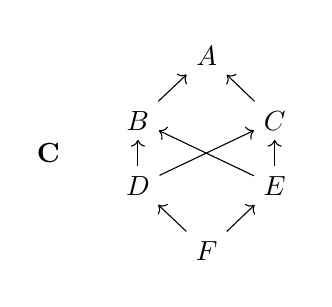
\begin{tikzpicture}
\matrix(A)[mymatrix,row sep=1em,column sep=1em]{
        & A & \\
      B &   & C \\
      D &   & E \\
        & F & \\
  };
  \path[draw,->]
    (A-2-1) edge (A-1-2)
    (A-2-3) edge (A-1-2)
    (A-3-1) edge (A-2-1)
    (A-3-3) edge (A-2-1)
    (A-3-1) edge (A-2-3)
    (A-3-3) edge (A-2-3)
    (A-4-2) edge (A-3-1)
    (A-4-2) edge (A-3-3);
  \node(cat)[left of=A,xshift=-1cm]{$\Cat{C}$};
\end{tikzpicture}
\end{center}

\begin{center}
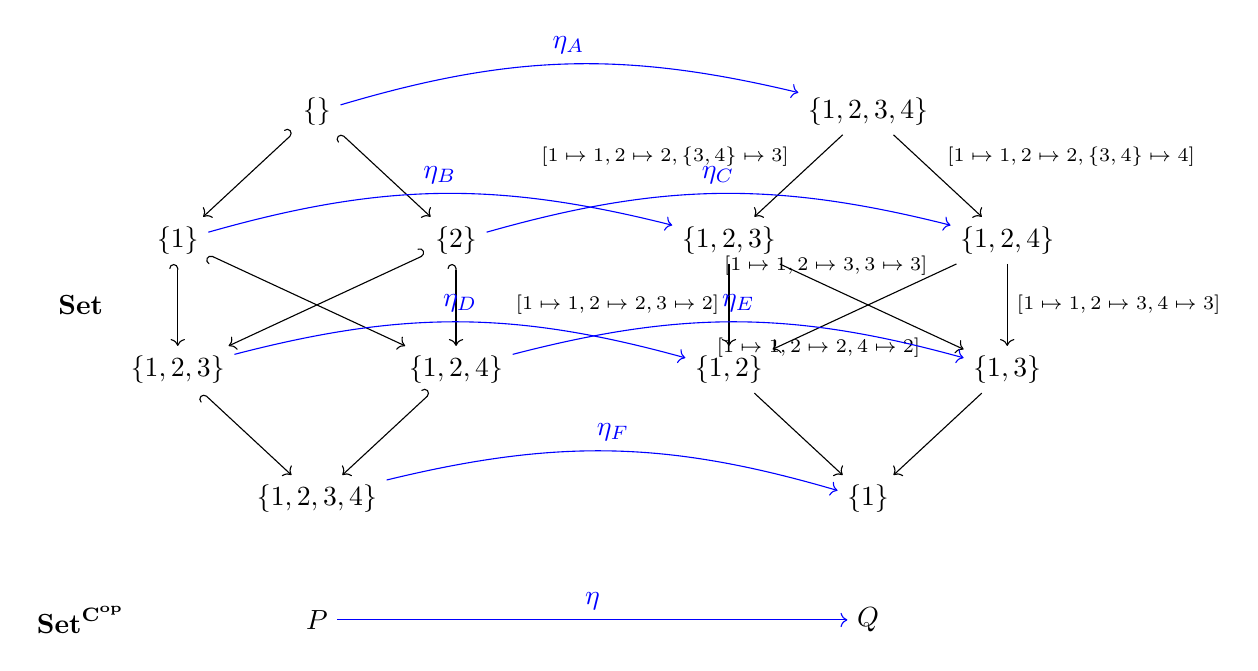
\begin{tikzpicture}[node distance=3cm]

  \node(set)[]{$\Set$};

  \matrix(B)[mymatrix,right of=set]{
              & \{\}        & \\
    \{1\}     &             & \{2\} \\
    \{1,2,3\} &             & \{1,2,4\} \\
              & \{1,2,3,4\} & \\
  };
  \path[draw,left hook->]
    (B-1-2) edge (B-2-1)
    (B-1-2) edge (B-2-3)
    (B-2-1) edge (B-3-1)
    (B-2-1) edge (B-3-3)
    (B-2-3) edge (B-3-1)
    (B-2-3) edge (B-3-3)
    (B-3-1) edge (B-4-2)
    (B-3-3) edge (B-4-2);

  \matrix(C)[mymatrix,right of=B,xshift=4cm]{
                & \{1,2,3,4\} & \\
      \{1,2,3\} &             & \{1,2,4\} \\
      \{1,2\}   &             & \{1,3\} \\
                & \{1\}       & \\
  };
  \path[draw,->,font=\scriptsize]
   (C-1-2) edge node[above left]{$[1 \mapsto 1,2 \mapsto 2, \{3,4\} \mapsto 3]$} (C-2-1)
   (C-1-2) edge node[above right]{$[1 \mapsto 1,2 \mapsto 2, \{3,4\} \mapsto 4]$} (C-2-3)
   (C-2-1) edge node[left]{$[1 \mapsto 1,2 \mapsto 2, 3 \mapsto 2]$} (C-3-1)
   (C-2-3) edge node[right]{$[1 \mapsto 1,2 \mapsto 3, 4 \mapsto 3]$} (C-3-3)
   (C-2-1) edge node[near start,above]{$[1 \mapsto 1,2 \mapsto 3, 3 \mapsto 3]$} (C-3-3)
   (C-2-3) edge node[near end,below]{$[1 \mapsto 1,2 \mapsto 2, 4 \mapsto 2]$} (C-3-1)
   (C-3-1) edge (C-4-2)
   (C-3-3) edge (C-4-2);

  \path[draw,->,bend left=15,blue]
    (B-1-2) edge node[above]{$\eta_A$}(C-1-2)
    (B-2-1) edge node[above]{$\eta_B$}(C-2-1)
    (B-2-3) edge node[above]{$\eta_C$}(C-2-3)
    (B-3-1) edge node[above]{$\eta_D$}(C-3-1)
    (B-3-3) edge node[above]{$\eta_E$}(C-3-3)
    (B-4-2) edge node[above]{$\eta_F$}(C-4-2);
  \node(presheaf)[below of=set,yshift=-1cm]{$\Set^{\Op{\Cat{C}}}$};
  \node(P) at (presheaf -| B) {$P$};
  \node(Q) at (presheaf -| C) {$Q$};
  \path[draw,->,blue] (P) edge node[above]{$\eta$} (Q);
\end{tikzpicture}
\end{center}
\end{example}

\section{Hom Functors and the Yoneda Embedding}
\label{sec:homfunctors}

\begin{definition}[Hom Functor]
  For a locally small category $\Cat{C}$, there is a functor $\mathrm{Hom}: \Op{\Cat{C}} \times \Cat{C} \rightarrow \Set$ defined on objects as $\mathrm{Hom}(A,B) \mapsto \Hom{\Cat{C}}{A}{B}$ and on arrows $f^\star : A \rightarrow A'$, $g: B \rightarrow B'$ as follows
  \begin{align*}
    \mathrm{Hom}(f^\star,g) : \Hom{\Cat{C}}{A}{B} & \rightarrow \Hom{\Cat{C}}{A'}{B'} \\
    h &\mapsto g \circ h \circ f
  \end{align*}
\end{definition}

\begin{lemma}[Hom Functors preserve limits]
  \label{lem:hompreserveslimits}
  $$\mathrm{Hom}(A,\lim{j \in \Cat{J}}F_j) \iso \lim{j \in \Cat{J}}(\mathrm{Hom}(A,F_j))$$
\end{lemma}

\begin{example}[Hom Functors preserve products]
  $$\mathrm{Hom}(A,B \times C) \iso \mathrm{Hom}(A,B) \times \mathrm{Hom}(A,C)$$
\end{example}

\begin{lemma}[Hom Functors map colimits to limits]
  \label{lem:hompreservescolimits}
  $$\mathrm{Hom}(\colim{j \in \Cat{J}}F_j,B) \iso \lim{j \in \Cat{J}}(\mathrm{Hom}(F_j,B))$$
\end{lemma}

\begin{example}[Hom Functors map coproducts to products]
  $$\mathrm{Hom}(A + B, C) \iso \mathrm{Hom}(A,C) \times \mathrm{Hom}(B,C)$$
\end{example}

\begin{definition}[Yoneda Embedding]
  The Yoneda embedding $Y: \Cat{C} \to \Presheaf{\Cat{C}}$ is the curried Hom functor, defined on objects by $Y(A) = \mathrm{Hom}(-,A)$ and on arrows $f:A \to B$ by
  \begin{align*}
    Y(f) = \mathrm{Hom}(-,f): \mathrm{Hom}(-,A) \to \mathrm{Hom}(-,B)
  \end{align*}
\end{definition}

\begin{lemma}[Yoneda Lemma]
  Let $F:\Op{\Cat{C}} \to \Set$ be a presheaf, then all natural transformation from the Yoneda embedding $Y(A)$ into $F$ are isomorphic to elements in $F(A)$:
  $$\Hom{\Presheaf{\Cat{C}}}{Y(A)}{F} \iso F(A)\qquad \text{natural in $A$ and $F$}$$
\end{lemma}

\clearpage
\begin{example}
  $\Hom{\Presheaf{\Cat{C}}}{\Hom{\Cat{C}}{-}{B}}{Q} \iso Q(B)$
\begin{center}
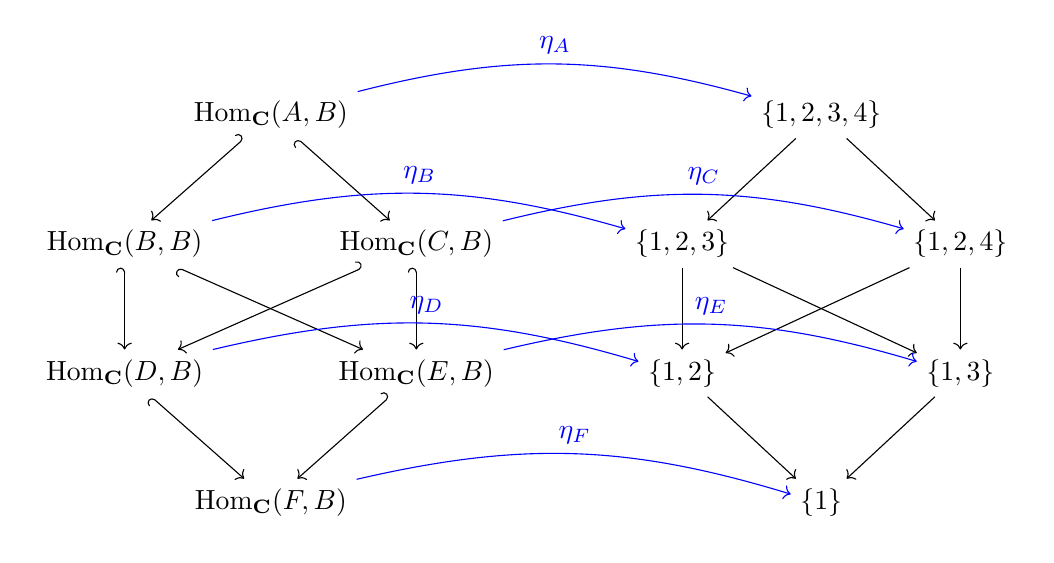
\begin{tikzpicture}[node distance=7cm]
  \matrix(B)[mymatrix,column sep=-1em]{
              & \Hom{\Cat{C}}{A}{B} & \\
    \Hom{\Cat{C}}{B}{B} & & \Hom{\Cat{C}}{C}{B} \\
    \Hom{\Cat{C}}{D}{B} & & \Hom{\Cat{C}}{E}{B} \\
              & \Hom{\Cat{C}}{F}{B} & \\
  };
  \path[draw,left hook->]
    (B-1-2) edge (B-2-1)
    (B-1-2) edge (B-2-3)
    (B-2-1) edge (B-3-1)
    (B-2-1) edge (B-3-3)
    (B-2-3) edge (B-3-1)
    (B-2-3) edge (B-3-3)
    (B-3-1) edge (B-4-2)
    (B-3-3) edge (B-4-2);

  \matrix(C)[mymatrix,right of=B]{
                & \{1,2,3,4\} & \\
      \{1,2,3\} &             & \{1,2,4\} \\
      \{1,2\}   &             & \{1,3\} \\
                & \{1\}       & \\
  };
  \path[draw,->,font=\scriptsize]
   (C-1-2) edge (C-2-1)
   (C-1-2) edge (C-2-3)
   (C-2-1) edge (C-3-1)
   (C-2-3) edge (C-3-3)
   (C-2-1) edge (C-3-3)
   (C-2-3) edge (C-3-1)
   (C-3-1) edge (C-4-2)
   (C-3-3) edge (C-4-2);

  \path[draw,->,bend left=15,blue]
    (B-1-2) edge node[above]{$\eta_A$}(C-1-2)
    (B-2-1) edge node[above]{$\eta_B$}(C-2-1)
    (B-2-3) edge node[above]{$\eta_C$}(C-2-3)
    (B-3-1) edge node[above]{$\eta_D$}(C-3-1)
    (B-3-3) edge node[above]{$\eta_E$}(C-3-3)
    (B-4-2) edge node[above]{$\eta_F$}(C-4-2);
\end{tikzpicture}
\end{center}
There are exactly three natural transformation from $\Hom{\Cat{C}}{-}{B}$ into $Q$, one for each element in $Q(B)$.
\end{example}

\begin{theorem} The Yoneda embedding is full and faithful.
  $$\Hom{\Cat{C}}{A}{B} = Y(B)(A) \iso \Hom{\Presheaf{\Cat{C}}}{Y(A)}{Y(B)}$$
\end{theorem}

\begin{corollary}[Yoneda Principle]
  $$Y(A) \iso Y(B) \implies A \iso B$$
\end{corollary}

\begin{example}
  Let us prove $(A^B)^C \iso A^{B \times C}$ using the Yoneda principle: $Y((A^B)^C) \iso Y(A^{B \times C})$.
  To that end, take any object $X \in \Cat{C}$, then we have the following isomorphism:
\begin{proof}
  \begin{align*}
    \Hom{\Cat{C}}{X}{(A^B)^C} & \iso \Hom{\Cat{C}}{X \times C}{A^B} \\
                              & \iso \Hom{\Cat{C}}{(X \times C) \times B}{A} \\
                              & \iso \Hom{\Cat{C}}{X \times (C \times B)}{A} \\
                              & \iso \Hom{\Cat{C}}{X}{A^{C \times B}} 
  \end{align*}
  All isomorphisms are natural in $X$ and hence the Yoneda principle applies.
\end{proof}
\end{example}

\clearpage
\section{Structure of the Presheaf Category}
\label{sec:structureofpresheafcategory}

\begin{lemma}[The presheaf category is complete]
  For any locally small category $\Cat{C}$, the presheaf category $\Presheaf{\Cat{C}}$ has all limits and limits are computed point-wise.
\begin{proof}
  Suppose we have a small index category $\Cat{J}$ and $F: \Cat{J} \to \Set^{\Op{\Cat{C}}}$.
  \begin{align*}
    (\lim{j \in \Cat{J}}F_j)(A) & \iso \Hom{\Presheaf{\Cat{C}}}{Y(A)}{\lim{j \in \Cat{J}}F_j}   && \text{by Yoneda} \\
                                & \iso \lim{j \in \Cat{J}}(\Hom{\Presheaf{\Cat{C}}}{Y(A)}{F_j}) && \text{by \autoref{lem:hompreserveslimits}} \\
                                & \iso \lim{j \in \Cat{J}}(F_j(A))                 && \text{by Yoneda} \\
  \end{align*}
\end{proof}
\end{lemma}

\begin{example}
  Let $P,Q: \Op{\Cat{C}} \to \Set$ be two presheafs, then the product of $P$ and $Q$ is calculated point-wise.
  $$(P \times Q)(A) \iso P(A) \times Q(A)$$
\end{example}

\begin{lemma}[The presheaf category is cocomplete]
  The presheaf category has all colimits and colimits are computed point-wise.
\end{lemma}

\begin{example}
  Let $P,Q: \Op{\Cat{C}} \to \Set$ be two presheafs, then the coproduct of $P$ and $Q$ is calculated point-wise.
  $$(P + Q)(A) \iso P(A) + Q(A)$$
\end{example}

\begin{lemma}[Density]
  \label{lem:density}
  For any small category $\Cat{C}$, every presheaf $P: \Op{\Cat{C}} \to \Set$ is a colimit of a Hom functor
  $$\colim{j \in \Cat{J}} Y(A_j) \iso P,$$ where $\Cat{J}$ is the category of elements of $P$, written $$\int_{\Cat{C}} P.$$
\end{lemma}

\begin{lemma}[The presheaf category is cartesian closed]
  We define the exponential $Q^P$ of two presheafs $P, Q: \Op{\Cat{C}} \to \Set$ as follows:
  \begin{align*}
    Q^P(A) &= \Hom{\Presheaf{\Cat{C}}}{Y(A) \times P}{Q} \\
    Q^P(f) &= \Hom{\Presheaf{\Cat{C}}}{Y(f) \times \id_P}{Q}
  \end{align*}
\begin{proof}
  We now show that $\Hom{\Presheaf{\Cat{C}}}{X}{Q^P} \iso \Hom{\Presheaf{\Cat{C}}}{X \times P}{Q}$.
  \begin{align*}
    \Hom{\Presheaf{\Cat{C}}}{X}{Q^P}
      &\iso \Hom{\Presheaf{\Cat{C}}}{\colim{j}Y(A_j)}{Q^P} && \text{(by \autoref{lem:density})} \\
      &\iso \lim{j} \Hom{\Presheaf{\Cat{C}}}{Y(A_j)}{Q^P} && \text{(by \autoref{lem:hompreservescolimits})} \\
      &\iso \lim{j} Q^P(A_j) && \text{(by Yoneda)} \\
      &\iso \lim{j} \Hom{\Presheaf{\Cat{C}}}{Y(A_j) \times P}{Q} && \text{(by definition)} \\
      &\iso \Hom{\Presheaf{\Cat{C}}}{\colim{j}(Y(A_j) \times P)}{Q} && \text{(by \autoref{lem:hompreservescolimits})} \\
      &\iso \Hom{\Presheaf{\Cat{C}}}{\colim{j}(Y(A_j)) \times P}{Q} && \text{(products preserve colimits)} \\
      &\iso \Hom{\Presheaf{\Cat{C}}}{X \times P}{Q} && \text{(by \autoref{lem:density})}
  \end{align*}
\end{proof}
\end{lemma}

\begin{theorem} The Yoneda embedding preserves all products and exponentials in $\Cat{C}$, i.e.
  \begin{align*}
    Y(A \times B) &\iso Y(A) \times Y(B) \\
    Y(B^A) &\iso Y(B)^{Y(A)}
  \end{align*}
\end{theorem}

\end{document}

%%% Local Variables:
%%% mode: latex
%%% TeX-master: t
%%% End:
